% !TEX root = ../preamble.tex
\section{Finding similar movies}
	\begin{figure}[H]
	\centering
	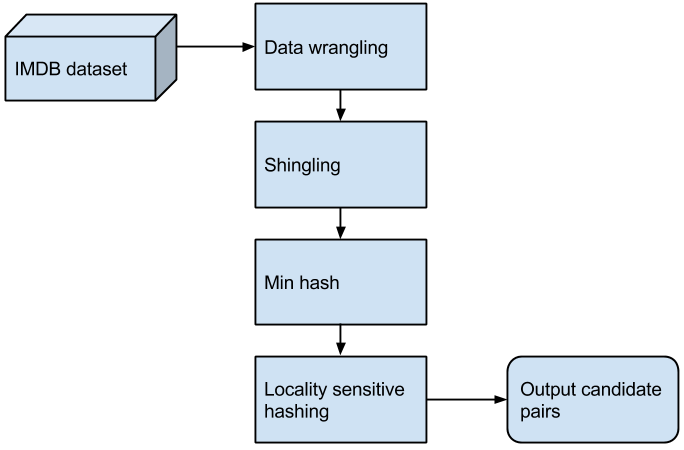
\includegraphics[width=250px]{img/Similaritysearchdiagram.png}
	\caption{The steps in similarity search} 
	\label{fig:p_graph}
\end{figure}
\subsection{Jaccard similarity}
Movie similarity is defined as Jaccard similarity of sets of a subset of movie attributes. Given two sets \textit{A} and \textit{B} the Jaccard similarity coefficient, \textit{j}, is defined as \(j = \frac{|A \cap B|}{|A \cup B|}\). \\ \\
The attributes considered when measuring similarity is title, genres, actors and directors. A set of actors is the identifiers of the actors having roles in the movie, a set of directors is the identifiers of the directors, and a set of genres is the names of the genres of the movie. The set that movie similarity is measured from is the union of all these sets as well as the title of the movie and is denoted \textit{C}.

\subsection{Min Hashing}
The purpose of Min Hashing is reducing the size the comparable movie representation, such that it still preserves its Jaccard similarity when being compared to other MinHashed objects, as well as making the representation suitable for locality-sensitive hashing.\\ \\
Min Hashing transforms \textit{C} to a signature, \(S\), which contains an integer for each hashing function used. The signature is generated by applying \textit{n} hash functions \(h_1(C), h_2(C),\ \dots\ , h_n(C)\) to the set, which produces a vector \([h_1(C), h_2(C),\ \dots\ , h_n(C)]\) of size \textit{n}, each element being the result of a hash function.\\ \\
The hash functions are defined using permutations. A permutation is a random ordering of all possible values of elements of \textit{C}, which is the union of all the sets that are to be compared. From a permutation, the hash value is computed by iterating through each element of the permutation, in the random order of the permutation. When an element is found that exists in \textit{C}, the hash function returns the index of that element in the ordering of the permutation.\\ \\
The reasoning for using Min Hash function to calculate signatures is that given two sets, \(C_1, C_2\), the probability of \(h(C_1) = h(C_2)\) is equal to the Jaccard similarity coefficient.
\begin{equation}
P(h(C_1) = h(C_2)) = \frac{|A \cap B|}{|A \cup B|}
\end{equation}
While Min Hashing produces a signature consuming significantly less space than \(C\), it stochastically preserves similarity.\\ \\
For the representation to be suitable for locality-sensitive hashing, each hash function has to be applied on each \(C_1, C_2,\ \dots\ , C_m\), producing \(m\) vectors \(S_1, S_2,\ \dots\ , S_m\), resulting in a matrix that is the input for the locality-sensitive hashing.

\begin{table}[h]
\begin{tabular}{l||l|l|l|l}
& \(S_1\) & \(S_2\) & \(S_3\) & \(S_4\) \\ \hline \hline
\(h_1(C)\) & 714 & 55 & 10034 & 183 \\ \hline
\(h_2(C)\) & 2 & 5213 & 3921 & 5213 \\ \hline
\(h_3(C)\) & 8322 & 377 & 475 & 15632
\end{tabular}
\centering
\caption{In this example, the 715'th element with index 714 of the permutation of the universal set for \(h_1(S)\) is the first element that the universal set and \(S_1\) had in common, starting from element 0.}
\end{table}

\subsection{Locality-sensitive hashing}
The purpose of locality-sensitive hashing is finding similar items, without examining each pair of items. The fundamental idea is to hash the signature of items several times, while only compare the items, of which the hash values collide. Item pairs, of which the hash value collide are called candidate pairs.\\ \\
The similarity threshold, \(t\), is the minimum similarity coefficient that a pair of items must have to be considered similar. The aim of LSH is to identify each pair with similarity greater than or equal to \(t\) as a candidate pair.\\ \\
Given a collection of signatures generated from the Min Hashing preprocessing step, each with size \(n\), the dimensions of the signature are grouped in \(b\) bands, each spanning \(r\) dimensions. The candidate pairs are found by hashing the subset of dimensions of each signature in each bands to buckets, such that two signatures with the same value in a band hashes to the same bucket. If a pair of item signatures hashes to the same bucket at least once, the items are considered candidate pairs. \\ \\

\begin{table}[h]
\begin{tabular}{l||l|l|l|l}
& \(S_1\) & \(S_2\) & \(S_3\) & \(S_4\) \\ \hline \hline
\(h_1(C)\) & \cellcolor[HTML]{FD6864} & \cellcolor[HTML]{FD6864}
 & \cellcolor[HTML]{FD6864} & \cellcolor[HTML]{FD6864} \\ \hline
\(h_2(C)\) & \cellcolor[HTML]{FD6864} & \cellcolor[HTML]{FD6864}
 & \cellcolor[HTML]{FD6864} & \cellcolor[HTML]{FD6864} \\ \hline
\(h_3(C)\) & \cellcolor[HTML]{38FFF8} & \cellcolor[HTML]{38FFF8}
 & \cellcolor[HTML]{38FFF8} & \cellcolor[HTML]{38FFF8} \\ \hline
\(h_4(C)\) & \cellcolor[HTML]{38FFF8} & \cellcolor[HTML]{38FFF8}
 & \cellcolor[HTML]{38FFF8} & \cellcolor[HTML]{38FFF8} \\ \hline
\(h_5(C)\) & \cellcolor[HTML]{9AFF99} & \cellcolor[HTML]{9AFF99}
 & \cellcolor[HTML]{9AFF99} & \cellcolor[HTML]{9AFF99} \\ \hline
\(h_6(C)\) & \cellcolor[HTML]{9AFF99} & \cellcolor[HTML]{9AFF99}
 & \cellcolor[HTML]{9AFF99} & \cellcolor[HTML]{9AFF99}
\end{tabular}
\centering
\caption{In this example the 6 rows has been divided into 3 bands with two rows each. The concrete results of the hash functions has been omitted.}
\end{table}

When the candidate pairs are found, their similarity is measured to determine whether they are actual pairs with similarity greater than or equal to \(t\). This method produces false negatives, and false positives in the sense that for some candidate pairs \(j<t\).

\subsubsection{Choosing the number of bands and rows}
The probability that two items will hash to the same bucket is a function of the similarity of the pair, the number of bands and the number of rows. A pair of items will hash to the same bucket of a band if the row values are equal, and the probability that a pair of row values are equal is \(j\). Hence the probability that a pair of items do not hash to the same bucket of one band is \(1-j^r\). The probability that the pair does not hash to the same bucket across all bands is \((1-j^r)^b\), and finally \(1-(1-j^r)^b\) is the probability that the pair is identified as a candidate pair.\\ \\
The function \(p(j) = 1-(1-j^r)^b\) is the connection between the probability that a pair is identified as a candidate pair and the similarity of the pair, \(j\). A higher number of bands clearly makes the probability larger that a pair is identified as a candidate pair, while a higher number of rows lowers this probability.\\ \\
\begin{figure}[H]
	\centering
	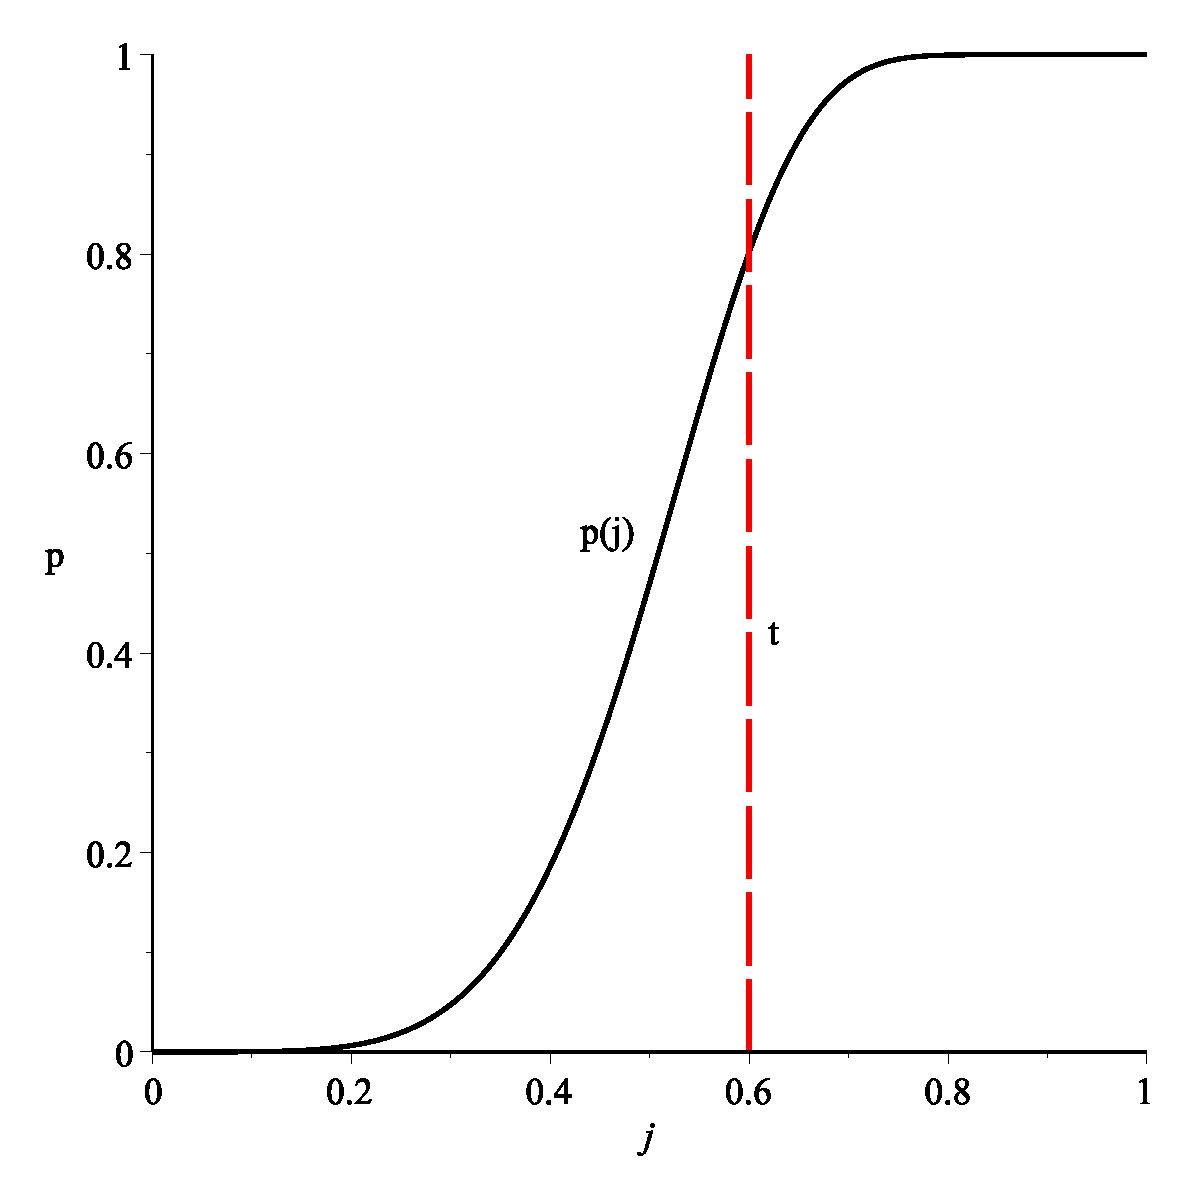
\includegraphics[width=250px]{img/pGraph.eps}
	\caption{The s-curve of \(p(j)\) with \(t = 0.6\), \(r = 5\) and \(b =20\)} 
	\label{fig:p_graph}
\end{figure}
The settings for \(b\) and \(r\) depends on the application of LSH. If the threshold is high, setting \(b\) and \(r\) to yield a low probability, might be reasonable. If the probability that a pair satisfying the threshold is identified as a candidate pair should be low, \(b\) should be increased and \(r\) lowered. Increasing b increases the fraction of false positives out of all \(n\) pairs, \(f_p\), and increasing \(r\) increases the fraction of false negatives, \(f_n\).\\ \\
To make a more precise statement on the connection between \(b\), \(r\), \(f_n\) and \(f_p\), an assumption on the distribution of item pairs has to be made. It is assumed that the distribution of items on \(j\) is continuously uniform in the interval \([0, 1]\), which is a strong assumption, because for our data set, the number of item pairs with \(j<0.2\) is much higher than the number of item pairs with \(j>0.8\).\\ \\
With a continuous uniform distribution, \(f_p\) can be estimated as the integral of \(p(j)\) from 0 to \(t\).
\[f_p = \int\limits_0^t\ p(j)\mathrm{d}j\]
To estimate \(f_n\), we subtract the entire area from \(t\) to \(1\) which is \(1-t\) with the integral of \(p(j)\) from \(t\) to \(1\).
\[f_n = (1-t)-\int\limits_t^1\ p(j)\mathrm{d}j\]
The continuous uniform distribution assumption makes the similarity \(j\) directly translatable to item pairs, and probability is over a large sample directly translatable to the fraction of item pairs returned as candidate pairs. The integral function estimates the product of item pairs and the fraction returned as candidate pairs.

\begin{figure}[H]
	\centering
	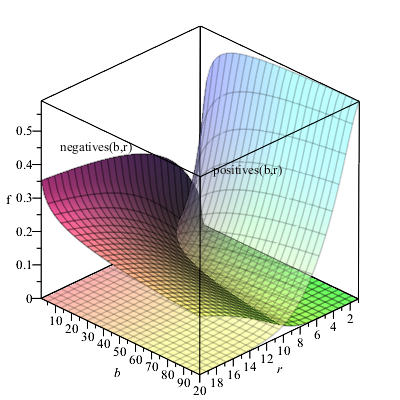
\includegraphics[width=290px]{img/falseGraph.jpg}
	\caption{The fraction of false positives or false negatives of all pairs, as a function of the number of rows and the number of bands with \(t=0.6\).}
	\label{fig:false_graph}
\end{figure}

Figure ~\ref{fig:false_graph} visualises the connection between \(b\), \(r\), \(f_n\) and \(f_p\). The connection is complicated, but it is apparent that the sum of \(f_n\) and \(f_p\) is reduced when \(b\) and \(r\) are increased. It is relevant to note that the uniform distribution assumption does make the fraction of false negatives seem larger and the number of false positives seem smaller than it is in a scenario where for a random pair \(Pr[j<0.5] > Pr[j>0.5]\), which is much more realistic.
\\
\\
\subsubsection{Time complexity of locality-sensitive hashing}
The time complexity of similarity search can be split into two parts, the preprocessing and the actual time to run a query after the preprocessing.\\
The preprocessing step hashes all N input points into L hashtables. This requires \(O(NLkt)\) time, as every input, must be put into all \(L\) hashtables and it takes \(kt\) time to do so, with \(t\) being the time to hash an input. The query step is 
now to hash all input points into their correct bucket and retreive all candidatepairs. \\
This is done over two stages. First; hashing all points into buckets take \(O(bNkt)\), since all input points is hashed as many times as there are bands. Next, all buckets is being checked if it contains any collisions between input points. This is a run through all the buckets with \(rN\) entries to look at, resulting in a running time of \(O(brN)\). This gives a total running time for the query \(O(bN(kt+r)\). \\
The wrangling of the dataset prior to preprocessing is not considered, as it has nothing to do with the actual algorithm.
